\section{Profiler Design}
\label{sec:design}

To demonstrate the feasibility and ease of identifying and distinguishing individual users on a WiFi network based solely on observed advertising and analytics HTTP cookies, BiscuitSpy is comprised of three main components: 
\begin{enumerate}
\item Capturer: A packet sniffing tool to capture any HTTP packet travelling through the network.
\item CookieBowl: A utility for collecting cookies and extracting the relevant cookies based on pre-defined criteria.
\item Profiler: A tool which parses the information from the extracted cookies to aggregate this data and build a user profile.
\end{enumerate}

The Capturer monitors the WiFi network for any HTTP request or response packets, and filters out any such packets which do not contain cookie the ``Cookie" or ``Set-Cookie" headers. 
Appropriate packets are then sent to the CookieBowl; for each captured packet, the CookieBowl first extracts the names and values of all the cookies contained within into a map data structure.
Next, the CookieBowl searches for a pre-defined set of advertising and analytics cookies, the \emph{profiling cookies}, among all collected cookies, and separates out these relevant cookies.

The Profiler, takes the map of found profiling cookies and parses the data found in each cookie's value. 
As discussed in Section \ref{sec:background}, BiscuitSpy uses two types of advertising/analytics cookies to build a user profile: (1) \emph{global cookies}, and (2) \emph{local cookies}.
Since the value of global cookies does not change across different visited websites, BiscuitSpy can cross-reference each appearance of such cookies allowing it to link two independent HTTP requests captured by the packet sniffer during a single BiscuitSpy session. 
At the same time, local cookies, which contain a per-domain unique user identifier for the entire \emph{lifetime} of the cookie (\textbf{NEEDS VERIFICATION: per session, or per lifetime}) allow BiscuitSpy to infer crucial user browsing behavior.
By combining common global and local ad and analytics cookies, we are able to track individual users throughout a single browsing session using global cookies while gathering browsing behavior information via the associated local cookies.
Figure \ref{fig:dataflow} shows the data flow between the various components of BiscuitSpy.

%TODO: change to say "found" profiling cookies
\begin{figure}[h]
\centering
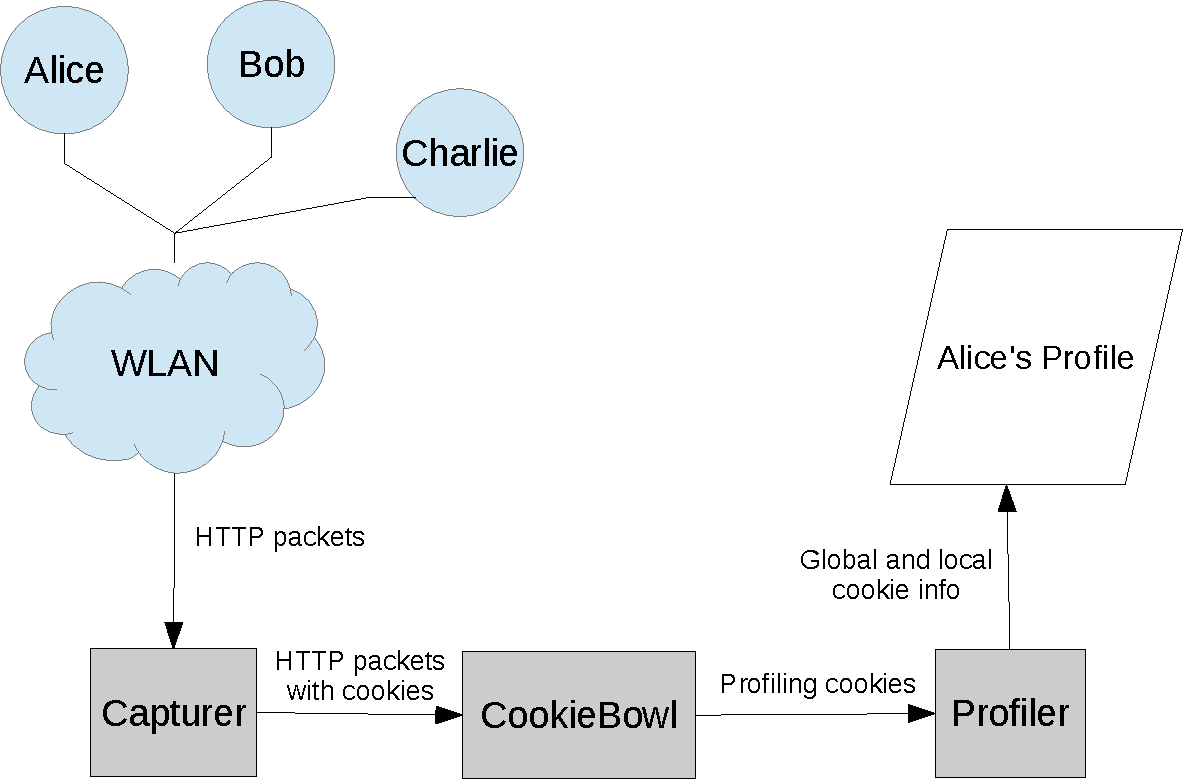
\includegraphics[scale=0.5]{./diagrams/dataflow.pdf}
\caption{The three main components of the BiscuitSpy tool and the data flow between them.}
\label{fig:dataflow}
\end{figure}

For each individual user identified by the Profiler, it stores the aggregated browsing behavior in a file for later offline analysis.
As cookies mostly contain encoded information, the Profiler converts this data to a human-readable format to facilitate the creation and reading of the profile.
One important note to make is that BiscuitSpy is limited by the type of data stored in the pre-defined profiling cookies.
Therefore, an analyst may not be able to learn personal information like a user's name or date of birth from her BiscuitSpy profile unless one of the profiling cookies contains an identifier, \emph{e.g.,} an email address, linkable to a real-world identity.
Nonetheless, even without such data, a user browsing profile could still be used to infer a user's habits or current issues in her life, as well as re-identify her during a later browsing session should she visit some or all of the same websites recorded in her initial profile.


\section{Implementation}
\label{sec:implementation}

We have implemented a basic command line-based BiscuitSpy prototype\footnote{The source code can be found at \url{http://github.com/naturegirl/BiscuitSpy.git}.} in Java (\textbf{ADD SLOC count?}) developed for Linux Ubuntu 12.04 LTS.
Our code is divided into three main packages: \texttt{cookies} which contains the CookieBowl as well as a general Cookie class, \texttt{cookies.definitions} which contains subclasses of Cookie, one for each profiling cookie, and \texttt{profiler} which contains both the Profiler, the Capturer, and a general Profile class.
Because the Capturer uses the \texttt{jnetpcap-1.3.0} library, a full Java implementation of the \texttt{pcap} API for capturing network traffic, we have bundled its source with the Profiler's to facilitate communication between the two classes.

The Profiler keeps a list of each Profile so that it can search through all Profiles seen so far and potentially annotate these with new information as it discovers cookies that belong to the same user. 
Before ending a BiscuitSpy session, the analyst can choose to save some or all profiles to separate files for later analysis.